\documentclass[11pt]{article}
\usepackage{fullpage,enumitem,tikz,graphicx,listings}
\usepackage{amsmath,amssymb,amsthm,graphicx,subcaption}
\usepackage[hyphens]{url}
\usepackage[hidelinks]{hyperref}
\hypersetup{breaklinks=true}

\usetikzlibrary{math}
\renewcommand{\baselinestretch}{1.5}
\allowdisplaybreaks[1]
\newtheorem{assumption}{Assumption}
\newtheorem{proposition}{Proposition}
\newtheorem{lemma}{Lemma}
\newtheorem{corollary}{Corollary}
\newtheorem{theorem}{Theorem}
\newtheorem{definition}{Definition}
\newtheorem{conjecture}{Conjecture}
\newtheorem{example}{Example}
\newtheorem{conj}{Conjecture}
\newtheorem{claim}{Claim}
\newtheorem{note}{Note}

\usepackage[a4paper,margin=0.8in,footskip=0.25in]{geometry}

\title{The Effects of Nonpharmaceutical Interventions\\ on the Spread of COVID-19 in Europe}
\author{Ming Fong, Seunghwan Lim, Peida Tian}

\begin{document}
\maketitle

\section{Problem Statement}
\begin{figure}[!hbt]
\centering
    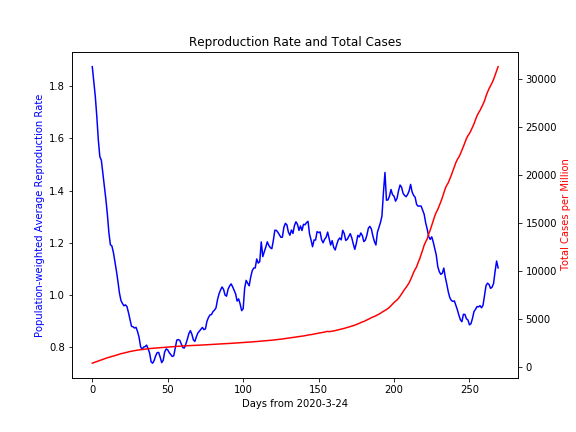
\includegraphics[width=0.6\textwidth]{reproduction_rate_and_total_cases.png}
    \caption{Total cases and reproduction rate in European countries}
    \label{fig:uk_ts_total_reproduction}
\end{figure}
\textbf{Our analysis set out to determine the effectiveness of various non-pharmaceutical response measures taken by governments to reduce the spread of COVID-19.} Contagiousness is one of the most important properties of a pandemic, and some research suggests that COVID-19 is even more contagious than SARS virus (\cite{liu2020}). We measure the spread of COVID-19 using effective reproduction rate, also commonly referred to as \textit{reproduction rate}.  Reproduction rate is ``the average number of secondary cases per infectious case in a population made up of both susceptible and non-susceptible hosts."\footnote{Health Knowledge, \url{https://www.healthknowledge.org.uk/public-health-textbook/research-methods/1a-epidemiology/epidemic-theory}}.  We also can see from Figure \ref{fig:uk_ts_total_reproduction} that reproduction rate is a good predictor of the total number of cases; as the reproduction rate increase from mid May, the total number of cases increases a accelerating speed. 

In response to the spread of COVID-19, many countries imposed various non-pharmaceutical interventions, which we refer as \textit{responses}, to slow down the spread of the virus. We analyze for 31 European countries on dates ranging from March 24th 2020 to December 18th 2020, and these countries imposed the total of 62 different responses in total during this period. However, it is still an open question whether these responses actually slow down the spread of the disease, and if so, how much they reduced the spread. Thus, in this project, we use various statistical models to predict the effect of the responses on the reproduction rates.

\section{Executive Summary}
\textbf{First, for each of the responses, we calculate how much they change the reproduction rate and the the number of days it takes to maximize this effect.} Figure \ref{fig:delay_eff} shows the effect and delay of each response to reproduction rate. Our model shows that adaptation of workplaces (\textit{AdaptationOfWorkplace}) is the most effective response: it reduced the reproduction rate by 0.45 in 3 days. However, this response was only implemented by by 6 countries (Czechia, Denmark, Netherlands, Poland, Spain, Sweden). Recommendations to close public transportation (\textit{ClosureOfPublicTransportPartial}) also reduced the reproduction rate by 0.37 in 15 days, but this was also only implemented by 3 countries (Ireland, Italy, Latvia). Limiting indoor/outdoor public gathering (\textit{BanOnAllEvents}) also turned out to be efficient, reducing the reproduction rate by 0.18 in 12 days. Czechia, Italy, Latvia, Netherlands, Poland, Spain, and Sweden were only ones that implemented at least 2 of these responses among 31 countries, and there was no country that implemented all 3 of these measures. This result implies that more European countries should implement these effective policies to slow down the spread of COVID-19

\begin{figure}[!hbt]
\centering
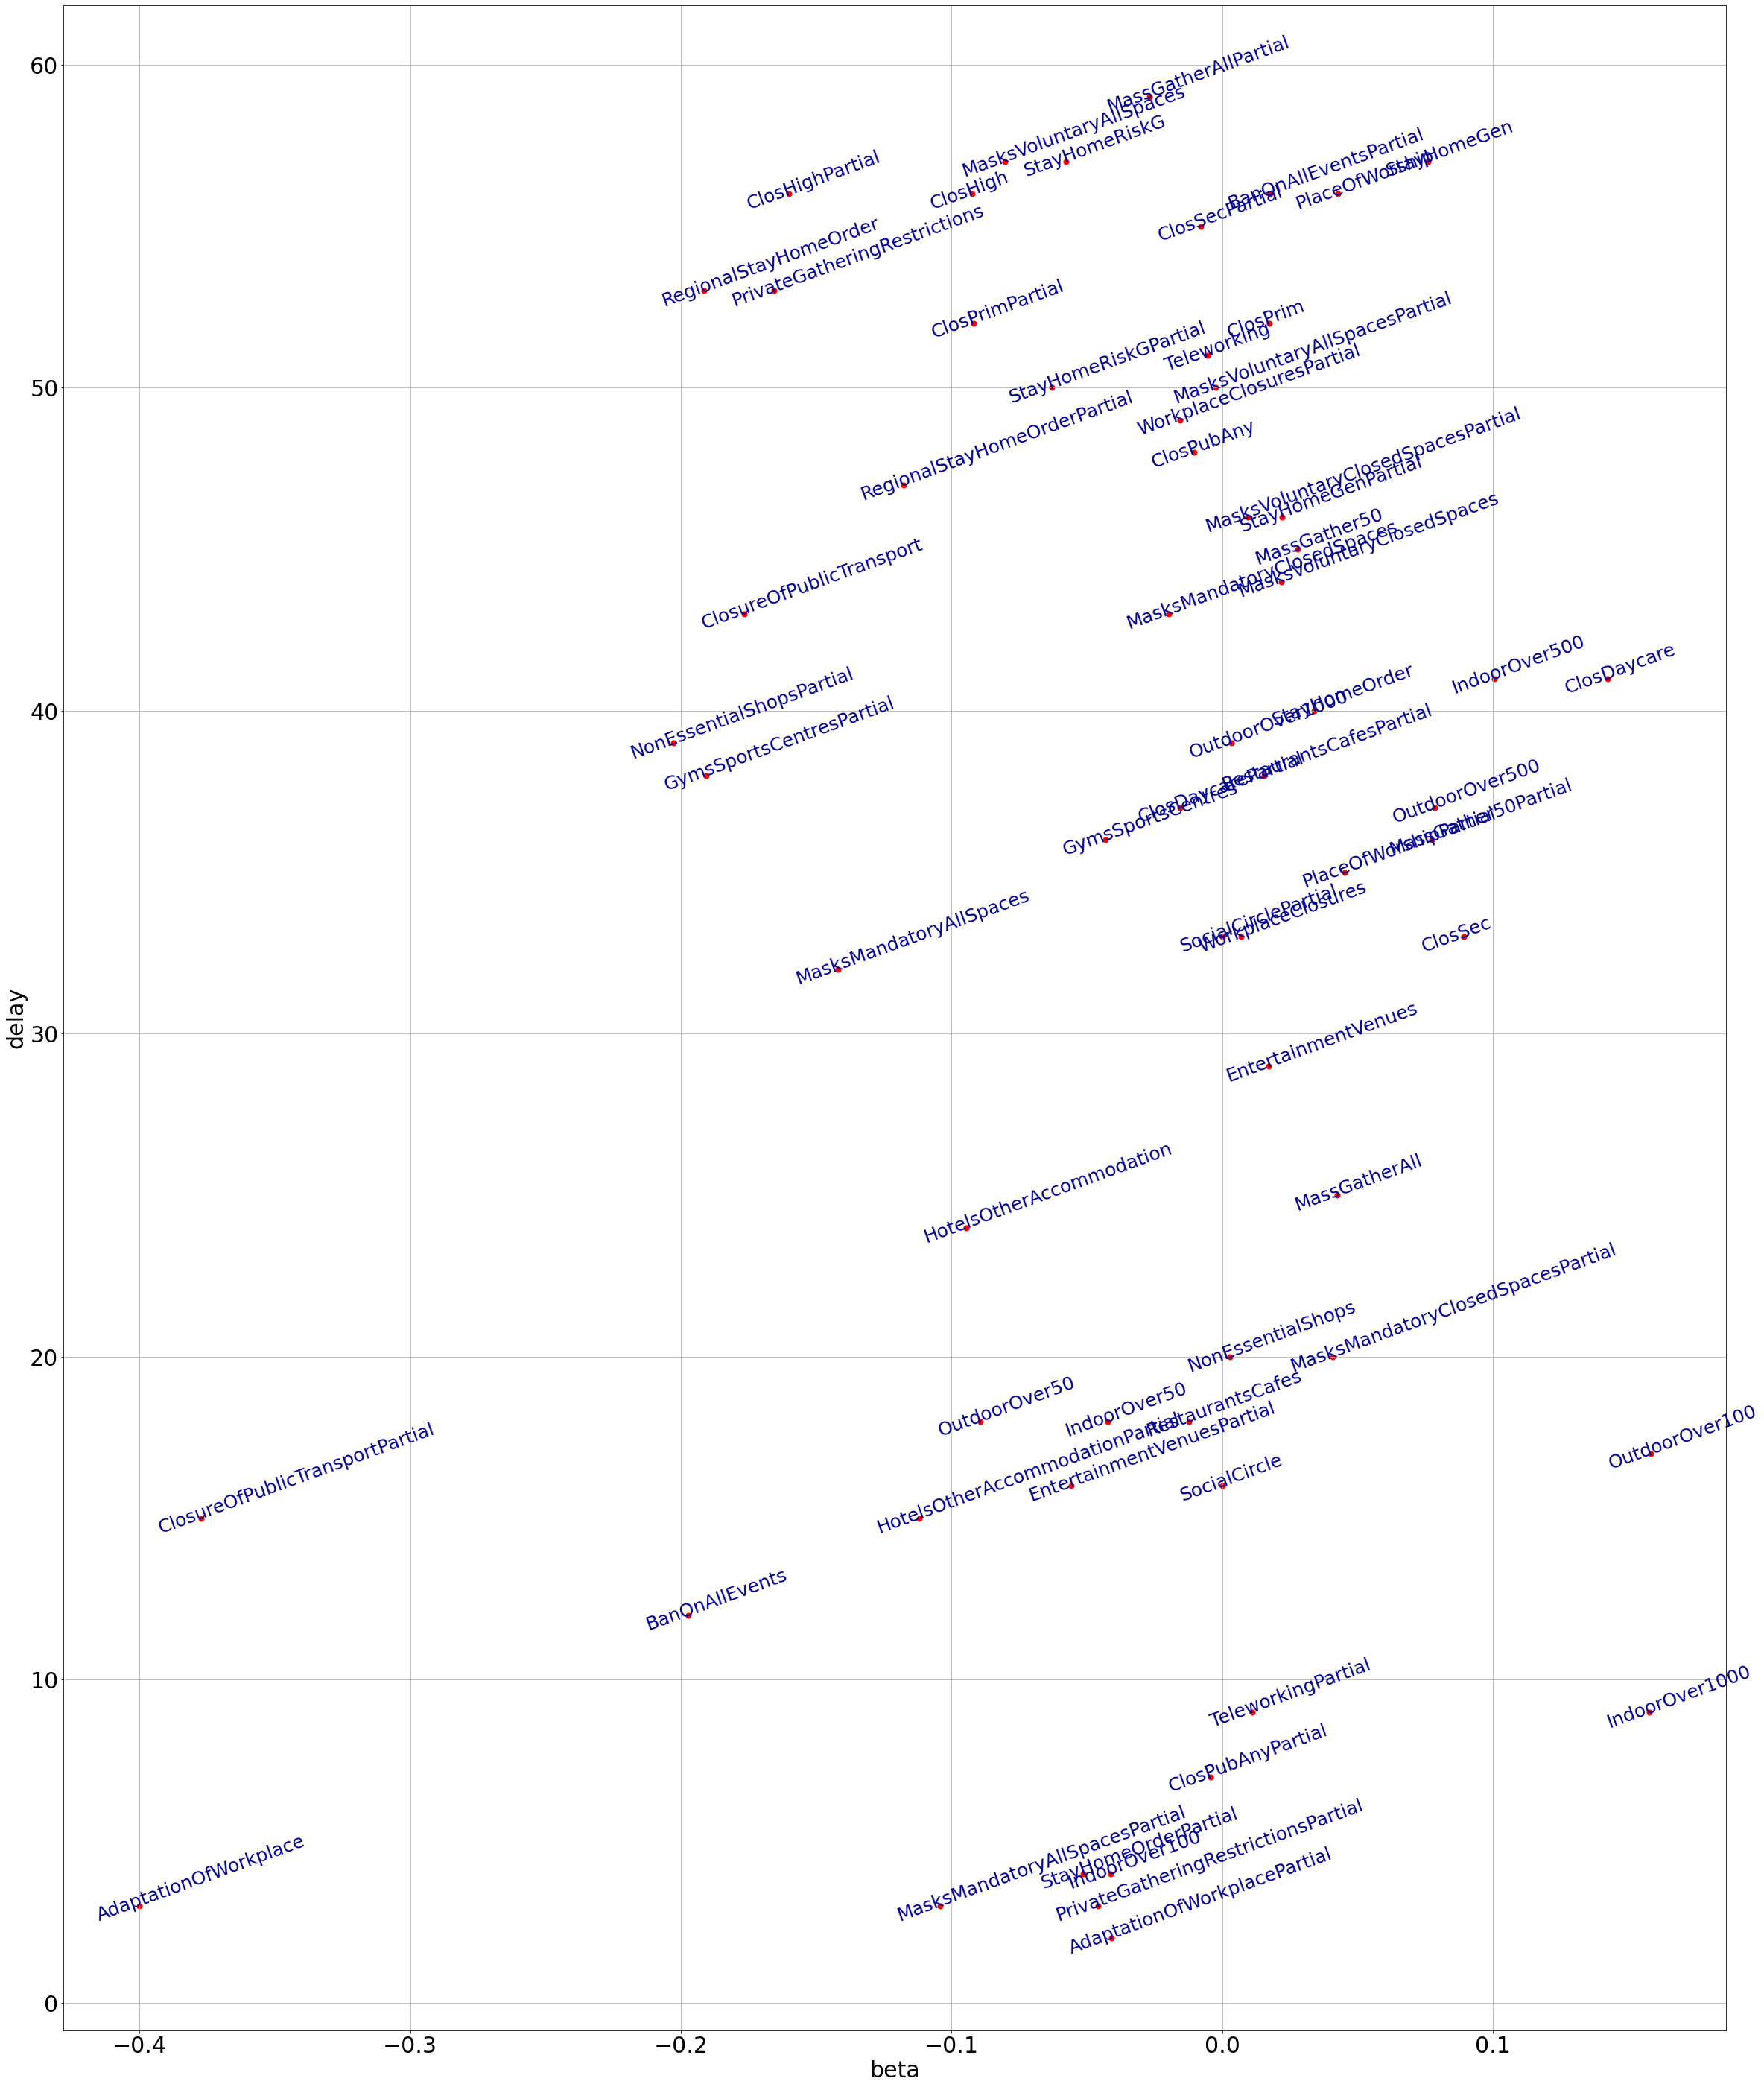
\includegraphics[width=0.5\textwidth]{delay_eff.png}
    \caption{The time-delay and effectiveness of response measures.}
    \label{fig:delay_eff}
\end{figure}

\textbf{Second, we train a neural-network model that predicts the change in response rate from different combinations of responses}. Our model trained on data from 25 countries and was tested on the remaining 6 countries to verify its accuracy. Figure \ref{fig:6_country_predictions} shows the results of these predictions. Our model generally follows the trends of actual reproduction rates in these 6 plots. Having verified the validity of our model, we propose a theoretical scenario for Sweden. Sweden is interesting because the Swedish government initially took very few responses to combat COVID. Although this strategy seemed promising at first, Swedish COVID rates eventually increased.

\textbf{What if Sweden implemented severe lockdown measures starting at day 1?} We can try and answer this question by modelling an extreme case where Sweden implements every type of response measure at all times. The prediction of this model is shown in figure \ref{fig:sweden_extreme_case}. From our prediction, if Sweden had imposed response measure from day 1, their initial reproduction rates would be much lower. Later Sweden eventually implements more measures, so their actual reproduction rates move closer to our predicted extreme case.

\begin{figure}[!h]
\centering
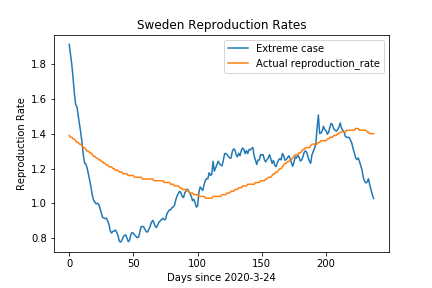
\includegraphics[width=0.6\textwidth]{test_country_predictions/sweden_extreme_case.png}
         \caption{Effectiveness ranking of response measures.}
         \label{fig:sweden_extreme_case}
\end{figure}

\section{Data and Summary Statistics}
We use the data from \textit{Our World in Data (OWID)} for demographics and daily COVID-19 data, such as number of total and new patients, positive rate, and effective reproduction rate. \textit{European Centre for Disease Prevention and Control (ECDC)} provides the list of responses taken by European countries, their starting dates, and their end dates. Thus, the data shows that responses taken by each of the 31 target countries\footnote{Austria, Belgium, Bulgaria, Croatia, Cyprus, Czechia, Denmark, Estonia, Finland, France, Germany, Greece, Hungary, Iceland, Ireland, Italy, Latvia, Lithuania, Luxembourg, Malta, Netherlands, Norway, Poland, Portugal, Romania, Slovakia, Slovenia, Spain, Sweden, Switzerland, United Kingdom (countries were in alphabetical order)} in each date between Match 24th 2020 to December 18th 2020. For each of the countries, OWID data provides 12 different of demographic data \footnote{population, population density, median age, Share of the population that is 65 years and older, Share of the population that is 70 years and older in 2015, GDP per capita, death rate from cardiovascular diseases in 2017, diabetes prevalence in 2017, share of women who smokes, share of men who smoke, hospital beds per thousand, life expectancy,human development index}. The total number of 62 different responses were taken by the countries during this time period.

Figure \ref{fig:hist_response_by_countries} shows the number of responses taken by each country, without counting duplicates. The average number of responses taken by countries is 22.87 with standard deviation of 7.86, and the median of the numbers of responses taken in 23. Czechia took 40 different responses, which is the largest number among 31 countries, and Croatia only took 8 different responses, which is the smallest. Figure \ref{fig:hist_response_frequencies} shows the number of countries that implemented each of the responses. The response taken by the most of number of countries was recommendation or unenforced order to close down restaurants, cafes, and bars (\textit{RestaurantsCafesPartial}), and 28 countries took this response. However, only Cyprus recommended the closure of workplaces (\textit{WorkplaceClosuresPartial}) and only Germany recommended to limit the size of social gathering (\textit{SocialCirclePartial}).

Figure \ref{fig:box_reproduction} shows the summary statistics of reproduction rate of countries from Mar 24th 2020 to December 18th 2020, and Figure \ref{fig:ts_reproduction} plots the reproduction rate over time for each country. We can observe that the distribution of reproduction rate is different across countries, and reproduction rate is cyclic. This implies that our model of predicting the effect of response should take account of this country-wise and time-wise effect.

\section{Model}
We denote a country with subscript $i$ and period with time $t$. The period is the number of days from the starting date, Match 24th 2020. For example, March 24th 2020 corresponds to $t=0$, and March 25th 2020 to $t=1$, and so forth. We model the reproduction rate as a function of time, response measures $\Theta$, and country-wise demographics $X$, and time delay $\tau$ as follows.
\begin{equation}
     r_{i,t+\tau} = f(t) + g(\Theta_{i,t},X_i).\label{eq:main_model}\tag{MODEL}
\end{equation}

Where $r_{i,t+\tau}$ is the reproduction rate of country $i$ at time $t+\tau$ and $f(t)$ is the temporal trend of the reproduction rate across the 31 countries. \textbf{Find the source between coronavirus and time.} $\Theta_{i,t}$ is a vector of indicators such that each element corresponds to one response. Thus, at time $t$, if country $i$ is implementing the $k$th response, the $k$th elements of $\Theta_{i,t}$ is equal to 1. Otherwise, the $k$th element of $\Theta_{i,t}$ is 0. $X_{i}$ is the country-wise demographics that are fixed throughout the entire time frame. Finally, $r_{i,t+\tau}$ is country $i$'s reproduction rate at time $t+\tau$. It may take some time for response measures to take effect on reproduction rate, and this delay is expressed as $\tau$. Later, we also consider the case where the time delays might vary for different response measures.  

We first run linear and LASSO regression on \eqref{eq:main_model} by making further assumptions about the functional form of $f$ and $g$ as follows.
\begin{gather}
    f(t) = b + a_1t + a_2t^2 + a_3t^3 + a_4 t^4 + a_5 t^5,\label{eq:lr_model1}\\
    g(\Theta_{i,t},X_i) = \mu\cdot\Theta_{i,t} + \lambda \cdot X_i + \delta\cdot I\label{eq:lr_model2}
\end{gather}
Figure \ref{fig:ts_reproduction} shows that there are 4 extreme points in the trend, so we first approximate $f(t)$ with a degree-5 polynomial. Note that the y-intercept of the polynomial, $b$, also works as the intercept of the whole regression. We assume that $g$ is a linear function of indicator for responses, $\Theta$, and demographic data $X$. Figure \ref{fig:box_reproduction} shows that the average number of reproduction rates varies by the countries, so we add country-wise indicator $I$ to capture this effect.

Second, instead of making a linearity assumption, we use a neural network to fit the function $g$. We re-write the equation \eqref{eq:main_model} as follows.
\begin{equation}
    r_{i,t} - f(t) = g(\Theta_{i,t},X_i).\label{eq:nn_model}
\end{equation}
Note the main focus here is function $g$. Thus, we first estimate the time trend $f$ using the population-weighted average of reproduction weights, $\bar{r}_t$, and use $r_{i,t} - \bar{r}_t$ as the dependent variable. For $g$, we do not use country-wise indicator so that we can divide train and test set by countries, as it will be explained in more detail later.

As a final note, we emphasize that our model does not provide the prediction of the future prediction model per se. Our main focus of analysis is predicting the effect of different responses on reproduction rate for counterfactual analysis. Thus, our model gives the prediction about the \textit{change} in reproduction rate if a country implements a set of responses rather than the absolute level of reproduction rate in the future. We will provide a counterfactual analysis to further clarify this point.

\section{Regression for Estimating the Effectiveness of Responses}
\subsection{Linear regression}
\begin{figure}[ht]
     \centering
     \begin{subfigure}[b]{0.45\textwidth}
         \centering
         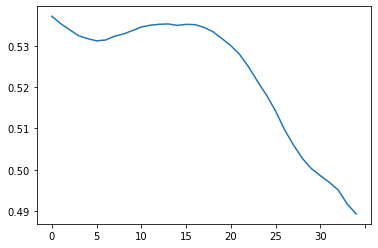
\includegraphics[width=\textwidth]{lr_bootstrap_mean.png}
         \caption{Mean of $R^2$'s from bootstrap method by $\tau$}
         \label{fig:lr_bootstrap_mean}
     \end{subfigure}
     \begin{subfigure}[b]{0.45\textwidth}
         \centering
         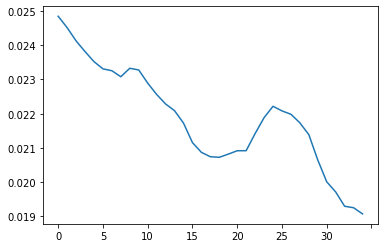
\includegraphics[width=\textwidth]{lr_bootstrap_std.png}
         \caption{Mean of $R^2$'s from bootstrap method by $\tau$}
         \label{fig:lr_bootstrap_std}
     \end{subfigure}
     \caption{Bootstrap method for linear regression.}
\end{figure}
In this section, we present the details of using Linear regression using the model \eqref{eq:main_model}, \eqref{eq:lr_model1}, and \eqref{eq:lr_model1}. We use bootstrap method to find the optimal delay $\tau$. We randomly sample 80 percent of the data and run linear regression for different values of tau ranging from 0 to 34. Then, we predict the reproduction rate for the rest of the data and calculate the $R^2$. We repeated this proces for 1,000 times, and observe the distribution of the $R^2$ for each $\tau$. We can see that when $\tau=14$, the mean of the $R^2$ is close to the maximum while attaining small standard deviation.

We can see that wearing mask mandatory in close spaces (\textit{MasksMandatoryClosedSpaces}) had the most impacts on decreasing reproduction rate. However, because it is one of the measure that was taken early, it is unclear whether this effect is due to timing.\footnote{Out of the 21 countries that implements this response, 14 countries implemented this measure by June.} Thus, in the next section, we vary the model and run more in-depth analysis for each of the responses.
\subsection{LASSO}
In this section, we present the details of using LASSO regression to rank the effectiveness of the response measures. The high level idea is to assign each response measure a weight, which we refer to as $\beta$-score. The $\beta$-score of a response measure indicates the reduction of reproduction rate when the corresponding response is in action. Hence, the more negative the $\beta$-score is, the more effective that response is. We then rank the response measures by their $\beta$-scores.    

Mathematically, LASSO is the specialization our general model in~\eqref{eq:main_model} to the linear case. Specifically, the reproduction rate $r_{i, t}$ of country $i$ at day $t$ is modeled by the $\beta$-score in the following way: for any fixed time-delay $\tau$, 
\begin{align}
    r_{i, t} (\beta, \tau) = (\beta_{\text{avg}} + \beta_{i}) + \sum_{\text{responses:} m}\beta_{m} \Theta^{(m)}_{i, t- \tau},
    \label{eq:lasso_model}
\end{align}
where     
\begin{itemize}
    \item $\tau$ is a given model parameter to indicate the time-delay between the starting date of the response and the time when the response affect the reproduction rate (later we choose optimal $\tau$ using the framework of Bayesian optimization, on top of LASSO);

    \item $\beta_{\text{avg}}$ is a parameter that reflects the reproduction rate in the case when no response is in action. The parameter $\beta_{i}$ captures the basic reproduction rate for a specific country $i$. 
        
    \item $\Theta_{i,t}^{(m)}$ is given by the data: $\Theta_{i,t}^{(m)} = 1$ when the response measure $m$ is active on day $t$ in country $i$, and $\Theta_{i,t}^{(m)} = 0$ otherwise.
\end{itemize}
Let $N_c, N_r$ be the number of countries in Europe and response measure, respectively. We then stack all the reproduction rate into a column vector, denoted by $R$, and collect all the $\beta_{\text{avg}}, \beta_i, \beta_{m}$ into a column vector $\beta$, that is 
\begin{align}
    \beta\triangleq \begin{bmatrix}
        \beta_{\text{avg}} &
        \beta_1 &
        \ldots &
        \beta_{N_c} &
        \beta_{\text{response} 1} &
        \ldots &
        \beta_{\text{response} N_r}
        \end{bmatrix}^\top,
\end{align}
where $\beta_{\text{response} i}$ is the $\beta$-score we assign to response $i$. The model~\eqref{eq:lasso_model} can be equivalently written in the compact form $R = M\cdot \beta$, where $M$ is a constant matrix constructed by collecting the coefficients of $\beta$ in~\eqref{eq:lasso_model}. Finally, let $R^{\text{(data)}}$ be the reproduction rate from the data, we have  $\text{LASSO}(\tau, \alpha)$: 
\begin{align}
        \min_{\beta}~ \|R^{\text{(data)}} - M\cdot \beta\|_2^2 + \alpha \|\beta\|_1
        \label{eq:lasso_form}\tag{$\text{LASSO}(\tau, \alpha)$}.
\end{align}
The parameter $\alpha$ regulates the number of nonzero elements in $\beta$. Figure~\ref{fig:eff_lasso} shows the ranking of the response measures based on the $\beta$-score from solving $\text{LASSO}(\tau = 32, \alpha = 5)$.


\begin{figure}[!hbt]
\centering
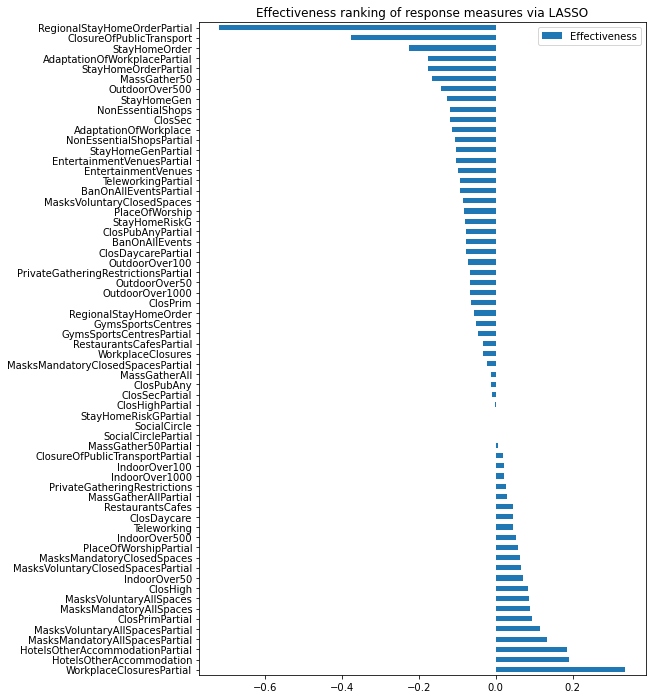
\includegraphics[width=0.8\textwidth]{eff_lasso.png}
         \caption{Effectiveness ranking of response measures.}
         \label{fig:eff_lasso}
\end{figure}

\subsection*{Hyperparameter tuning using Bayesian optimization:} We also apply Bayesian optimization to choose the optimal $(\tau^\star = 32, \alpha^\star = 5)$ to minimize the prediction error on the test set (which is 0.1 fraction of the whole dataset). The $\beta$-scores are shown in Figure~\ref{fig:eff_lasso}. 

\subsection*{Time-delays that vary for different response measures:} In this subsection, we explore the following aspect of response measures: \textbf{which response measures has the least delay to be effective?} To do so, we slightly modify the $\text{LASSO}(\tau, \alpha)$ to $\text{LASSO}(\tau_1,...\tau_{N_r}, \alpha)$, where $\tau_m$ is the time-delay associated to response measure $m$. We then apply Bayesian optimization on top of $\text{LASSO}(\tau_1,...\tau_{N_r}, \alpha)$ to choose the optimal $\tau^\star_m$ for each response $m$. We then rank the response measures by their corresponding $\tau^\star_m$. The result is shown in Figure~\ref{fig:delay_lasso}. As one can see, AdaptationOfWorkplacePartial, AdaptationOfWorkplace, MasksMandatoryAllSpacePartial are the top-three that has the least delays $\tau^\star = 3$. We also present a scatter plot in Figure~\ref{fig:delay_eff}. 
\begin{figure}[!hbt]
\centering
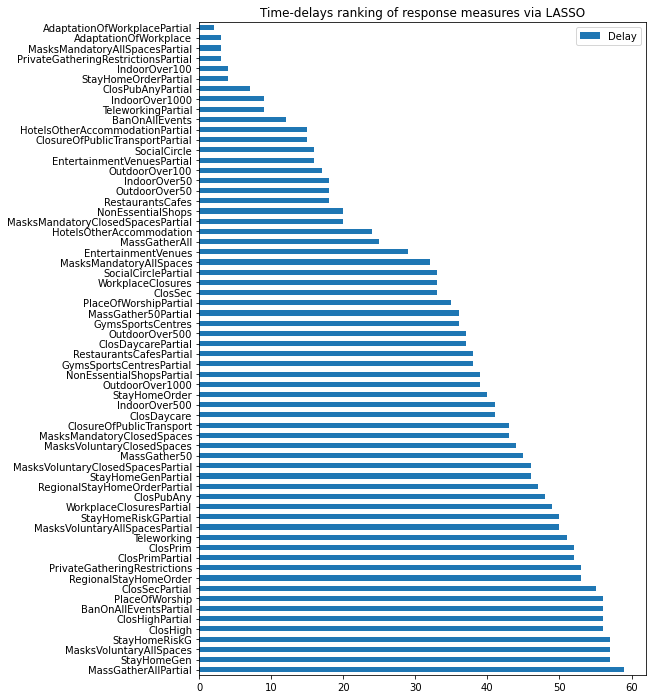
\includegraphics[width=0.8\textwidth]{delay_lasso.png}
         \caption{Time-delay ranking of response measures.}
         \label{fig:delay_lasso}
\end{figure}

\section{Neural Networks for Estimating the Effectiveness of Responses}
In order to better generalize $g(\Theta_{i,t},X_i)$ and estimate $\Delta r_{i,t}$, we implement a sequential neural network. Our input layer consists of the government responses currently in effect and the demographics of the country. Each row represents the state of one country on one date. We split out dataset into training and testing sets by randomly selecting 24 countries to train on and using the remaining 6\footnote{Finland, France, Italy, Lithuania, Portugal, Spain} to validate our model.

To best capture the effect of government responses, we apply a time shift of $32$ days using the optimal value of $\tau$ we calculated previously. Intuitively, this value represents the average time a certain government response will have a maximum effect in reducing reproduction rate. Thus we will have the best accuracy predicting $\Delta r_{i,t}$ $32$ days after a given day of responses.

Our model is implemented with Tensorflow and Keras. Our study of various model architectures found that the following simple architecture performed the best:

\begin{itemize}
    \item Input layer ($\Theta_{i,t},X_i$)
    \item Dense layer (64 Nodes)
    \item Dropout Layer
    \item Dense Layer (64 Nodes)
    \item Dropout layer
    \item Dense layer (1 Node)
\end{itemize}

Training and validation loss for 24 randomly selected countries is shown in figure  \ref{fig:delta_reproduction_rate_model_loss}.

\begin{figure}[!htb]
     \centering
     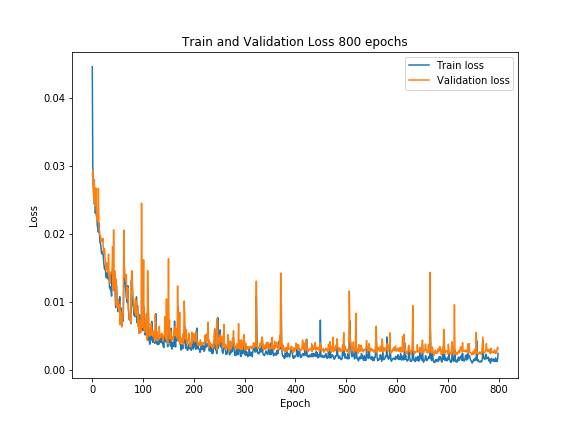
\includegraphics[width=0.6\textwidth]{delta_reproduction_rate_model_loss.png}
     \caption{Model loss for predicting $\Delta r_{i,t}$}
     \label{fig:delta_reproduction_rate_model_loss}
\end{figure}

We can evaluate the accuracy of our model first by calculating the root-mean-squared error (RMSE) of our predicted $\Delta r_{i,t}$ values and the actual values given in the dataset.

$$\text{RMSE}(\Delta r_{\text{pred}} - \Delta r_{\text{real}}) = \sqrt{\frac{1}{n}\sum_{i=1}^{n}(\Delta r_{\text{pred}} - \Delta r_{\text{real}})^{2}} = 0.1470799$$

This value is hard to understand intuitively, so we can visualize the accuracy of our predicted $\Delta r_{i,t}$ by adding the population-weighted European mean $f(t)$ to our predicted value and plotting it against actual $r_{i,t}$ values. We do this for each of the 6 countries from our testing dataset in Figure \ref{fig:6_country_predictions}.

\begin{figure}[!hbt]
    \centering
    \subfloat[Finland]{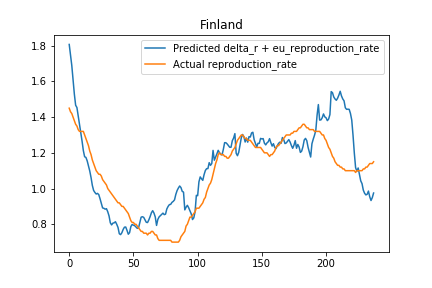
\includegraphics[width=8cm]{test_country_predictions/Finland_predictions.png}}\hfil
    \subfloat[France]{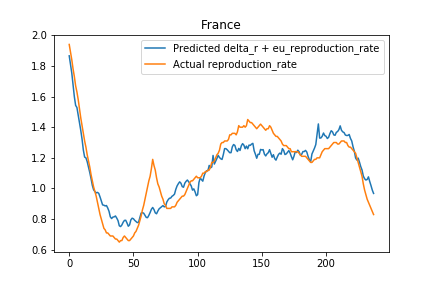
\includegraphics[width=8cm]{test_country_predictions/France_predictions.png}}\hfil
    \subfloat[Italy]{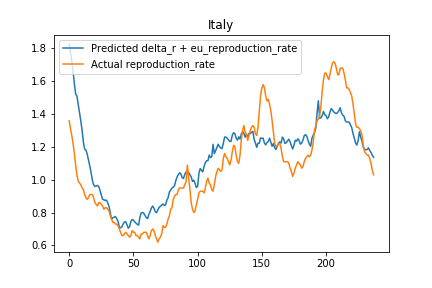
\includegraphics[width=8cm]{test_country_predictions/Italy_predictions.png}}\hfil
    \subfloat[Lithuania]{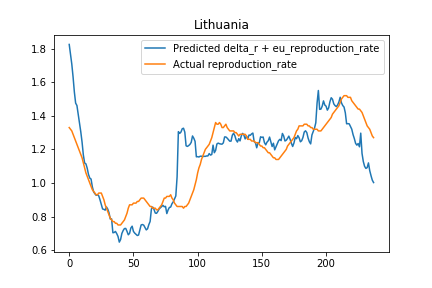
\includegraphics[width=8cm]{test_country_predictions/Lithuania_predictions.png}}\hfil
    \subfloat[Portugal]{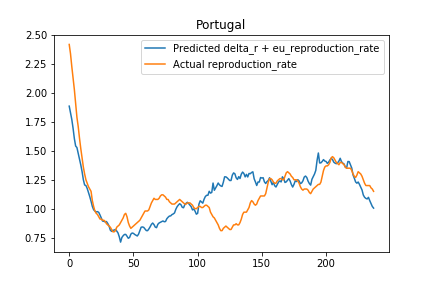
\includegraphics[width=8cm]{test_country_predictions/Portugal_predictions.png}}\hfil
    \subfloat[Spain]{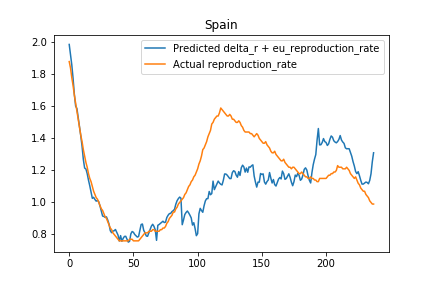
\includegraphics[width=8cm]{test_country_predictions/Spain_predictions.png}}
    \caption{Our predicted $\Delta r_{i,t} + f(t)$ plotted against actual values of $r_{i,t}$ for the 6 countries in the testing dataset}\label{fig:6_country_predictions}
\end{figure}
\nocite{*}
\bibliographystyle{acm}
\bibliography{datathon_reference.bib}
\newpage

\appendix
\section{Figures}\label{appendix:figure}
\begin{figure}[h]
     \centering
     \begin{subfigure}[b]{0.4\textwidth}
         \centering
         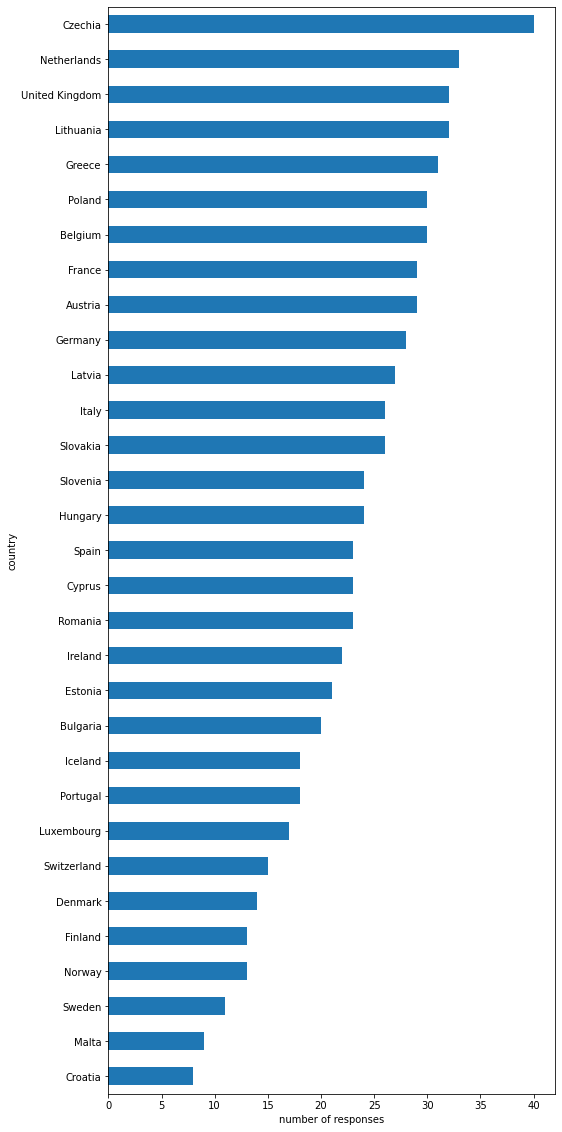
\includegraphics[width=\textwidth]{hist_response_by_countries.png}
         \caption{Number of responses for each country}
         \label{fig:hist_response_by_countries}
     \end{subfigure}
     \begin{subfigure}[b]{0.475\textwidth}
         \centering
         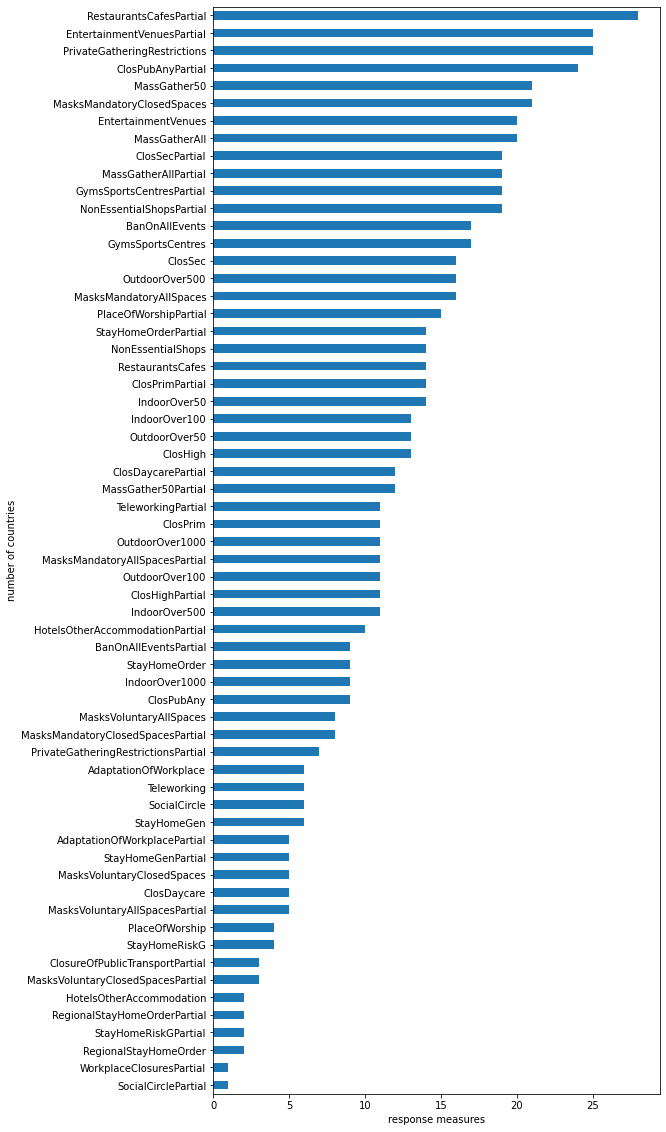
\includegraphics[width=\textwidth]{hist_response_frequencies.png}
         \caption{Number of countries for each response}
         \label{fig:hist_response_frequencies}
     \end{subfigure}
     \caption{The countries' responses to COVID-19.}
\end{figure}
\begin{figure}[h]
     \centering
     \begin{subfigure}[b]{0.8\textwidth}
         \centering
         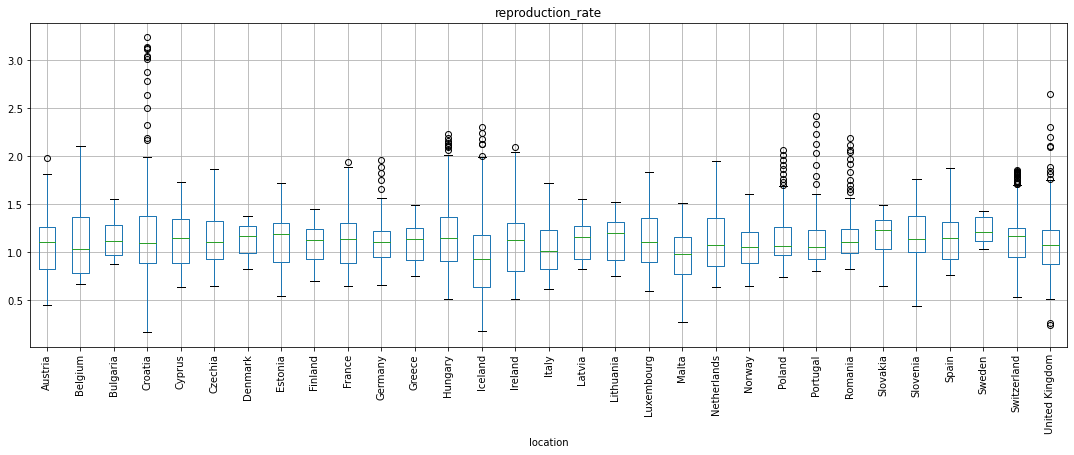
\includegraphics[width=\textwidth]{box_reproduction.png}
         \caption{Summary statistics for reproduction rate by countries}
         \label{fig:box_reproduction}
     \end{subfigure}
     \begin{subfigure}[b]{0.8\textwidth}
         \centering
         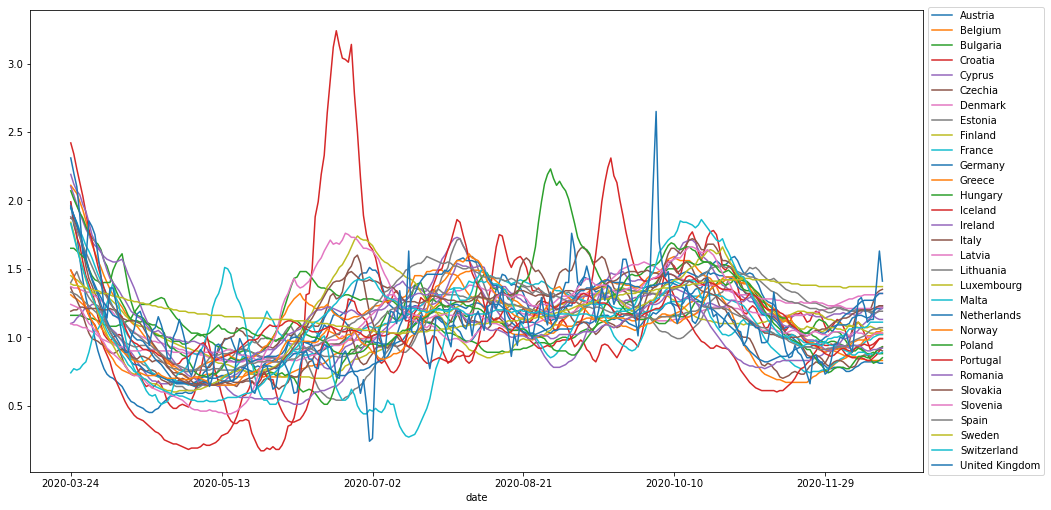
\includegraphics[width=\textwidth]{ts_reproduction.png}
         \caption{Reproduction rate by countries over time}
         \label{fig:ts_reproduction}
     \end{subfigure}
     \caption{Reproduction rate by countries from March 24th 2020 to November 18th 2020.}
\end{figure}
\begin{figure}[h]
    \centering
    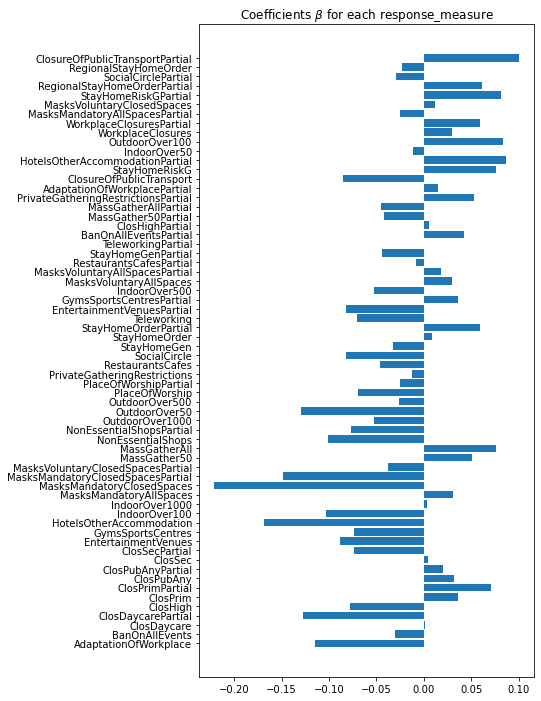
\includegraphics[width=0.7\textwidth]{lr_coefficients.png}
    \caption{Coefficients from linear regression for $\tau=14$}
    \label{fig:my_label}
\end{figure}
\end{document}
